% !TEX root = ../../../I4PRJ, Grp3 - Rapport.tex
\subsection{Model og Presenter}
Præsentationslaget består af interfaces til presenters og views, samt konkrete presenter-klasser. View interfaces specificeres af de tilhørende presenter-klasser.

\subsubsection{Design}
På figur~\ref{fig:application_isignupview} ses klassediagrammet for ISignUpView-interfacet.

\begin{figure}
\centering
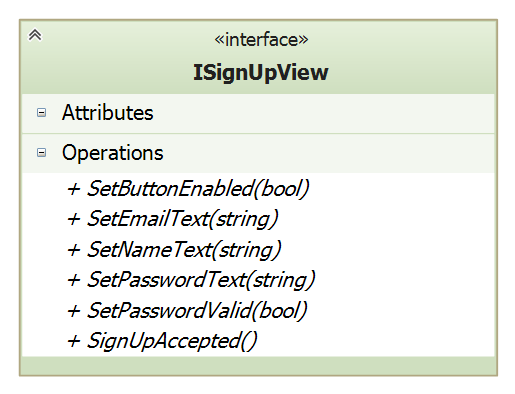
\includegraphics[width=0.4\linewidth]{figs/design/application_isignupview}
\caption{ISignUpView}
\label{fig:application_isignupview}
\end{figure}

Det konkrete signup view i hver platformspecifikke applikation implementerer view-interfacet og instantiere den tilhørende controller, hvis interface- og klassedesign ses på figur~\ref{fig:application_isignupviewcontroller}.

\begin{figure}
\centering
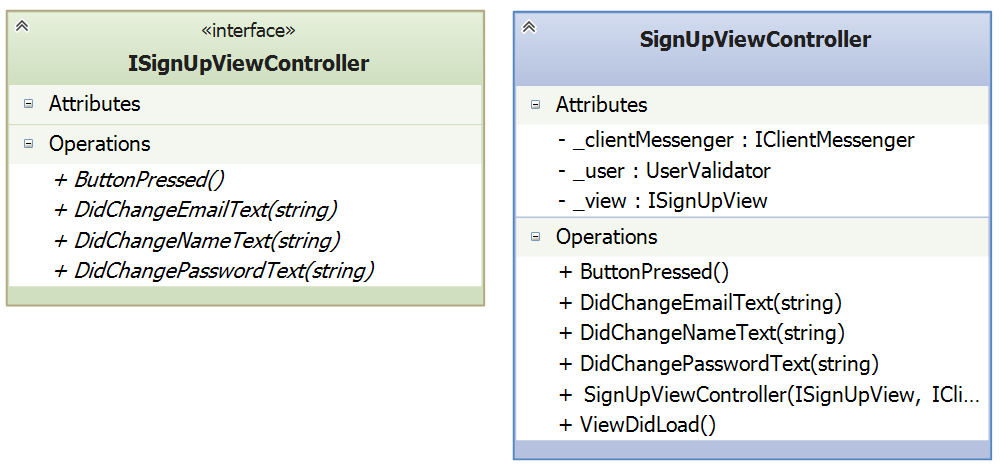
\includegraphics[width=0.7\linewidth]{figs/design/application_signupviewcontrollerandinterface}
\caption{ISignUpViewController og SignUpViewController}
\label{fig:application_isignupviewcontroller}
\end{figure}

Figur~\ref{fig:application_isignupviewcontroller} viser også, at den konkrete klasse indeholder flere metoder og attributter, som binder den konkrete klasse sammen med modellen. Modellen i applikationslaget består delvist af valideringslogik og klasser til kommunikation med resten af systemet. Det er attributter som \_clientMessenger, som er klienten, der kommunikerer med serveren, og \_user af typen UserValidater, der validerer om brugerinformationen er gyldig.

Den user story, der omhandler visning af målinger, har ført til designet af følgende presenter-klasse.

\begin{figure}
\centering
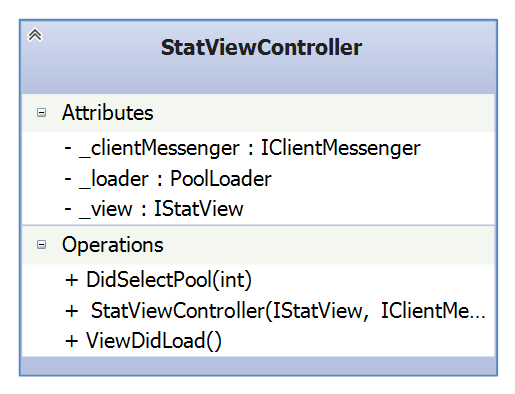
\includegraphics[width=0.35\linewidth]{figs/design/application_statviewcontroller}
\caption{StatViewController konkret klasse}
\label{fig:application_statviewcontroller}
\end{figure}

Største delen af modellaget ligger i Forbindelse, fordi det indgår i client-server arkitekturen. Se afsnit~\ref{sec:Connectiontier}, for mere information.

For yderligere forklaring se dokumentation afsnit Applikationslaget under Design.